\section{Anhang}
\subsection{Testergebnisse}

\subsection{Abmessungen}

\subsection{Datenblattauszüge}

\textcolor{blue}{Im Anhang befinden sich weitere Detailinformationen des Projekts wie\\
•	Datenblattauszüge, Fertigungsunterlagen (PCB-Layouts, Gehäusezeichnungen, 3D-Druckunterlagen, Montageanleitungen,…) etc.\\
•	sämtliche geforderten Projektmanagementdokumente\\
•	ein Businessplan (optional)
}

\subsection{Projektmanagement}
\textcolor{blue}{In diesem Kapitel soll auf das Projektmanagement des Projektes eingegangen werden. Zu Beginn empfiehlt es sich, die einzelnen Bereiche des Projektmanagements zu erklären und anschließend in einzelnen Kapiteln zu behandeln.}

\subsubsection{Aufgabenstellung des Gesamtprojekts}
\textcolor{blue}{Fügen Sie an dieser Stelle den Text der genehmigten Aufgabenstellung ein, der in die Diplomarbeitsdatenbank  eingegeben wurde.}

\subsubsection{Scrum-Projektplan}
\textcolor{blue}{Fügen Sie hier den vollständigen Scrum-Projektplan, wobei die Nummern der Tasks mit der Arbeitszeitaufzeichnung übereinstimmen müssen. Der Scrum-Projektplan kann auf mehrere Seiten aufgeteilt werden.}

\bgroup
    \centering
    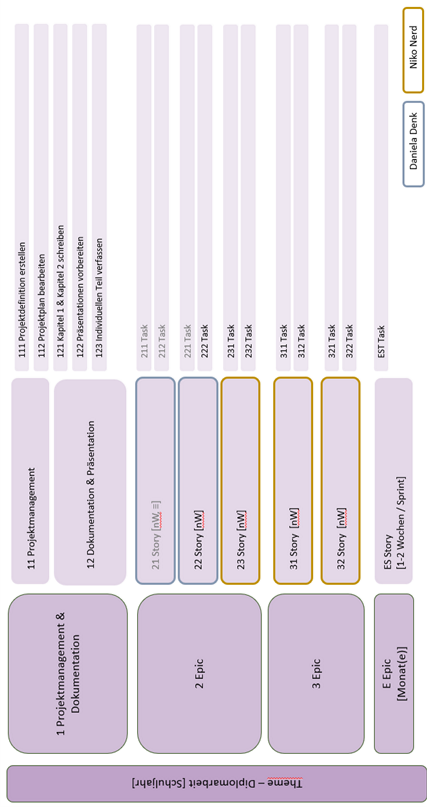
\includegraphics[width=0.6\textwidth]{Scrum_Projektplan_mit_Tasks.png}
    \captionof{figure}{Scrum Projektplan mit Tasks}
\egroup

\newpage
\subsubsection{Terminplanung}

\newpage

\subsubsection{Arbeitspakete}

\paragraph{Maschinenbau (Simbürger)}
\begin{itemize}
    \item Konzeptionierung des Gesamtsystem
    \item CAD - Planung
    \item Komponentenfertigung
    \item Aufbau 
\end{itemize}

\paragraph{Softwareentwicklung (Simbürger)}
\begin{itemize}
    \item Benutzeroberfläche
    \item Warehouse Management System
    \item Datenbanken
\end{itemize}




\newpage

\subsection{Inbetriebnahme}
\color{blue}
Nachdem typische Projekte aus mehreren Komponenten bestehen, ist es oft nicht trivial die einzelnen Komponenten korrekt zu konfigurieren und das Gesamtsystem in Betrieb zu nehmen. In diesem Kapitel soll eine vollständige, präzise und trotzdem möglichst kompak-te Anleitung zur Inbetriebnahme des Systems dargelegt werden. Die Schritte sollen in dem Detailgrad beschrieben werden, dass ein durchschnittlicher Schüler des vierten Jahrganges das Projekt in Betrieb nehmen kann. Exemplarisch sollten Punkte wie die folgenden be-handelt werden – die Aufzählung ist nicht vollständig):
\begin{itemize}
    \item Treiberinstallationen und Systemkonfigurationen
    \item Zu empfehlen wäre bei Server-Installationen ein Setup-Script, welches auf einem vordefinierten Docker-container aufbaut.
    \item Welche Schritte sind notwendig, um das Projekt mit dem vorhandenen Code / Schaltplänen (auf GIT, CD, Netzlaufwerk, etc.) in Betrieb zu nehmen.
    \item Bei Schaltungen mit mehreren Platinen muss beschrieben werden, wie diese mit-einander verbunden werden müssen.
\end{itemize}
\color{black}

\newpage
\subsection{Kostenaufstellung}
\textcolor{blue}{Für die Kalkulation im Gesamtprojekt sind folgende Kosten zu erfassen: \\
•	Kosten für Material (Hard- und Software)\\
•	externe Kosten (z.B.: Zukauf von Sensoren, Funkmodule, spezielle Entwicklungsum-gebungen, etc.) 
}
\begin{figure}[h]
    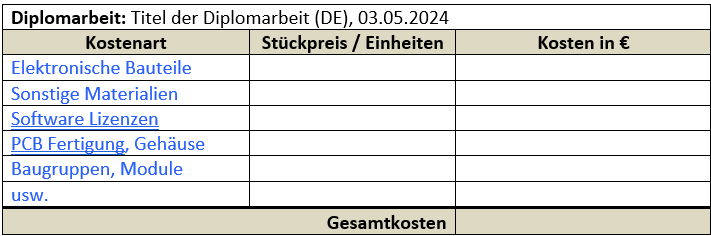
\includegraphics[width=0.8\textwidth]{Kostenaufstellung.png}
    \centering
    \caption{Kostenaufstellung}
\end{figure}

\newpage
\subsection{Besprechungsprotokolle}
%include pdf file as image, on howl page with label
\begin{figure}[H]
    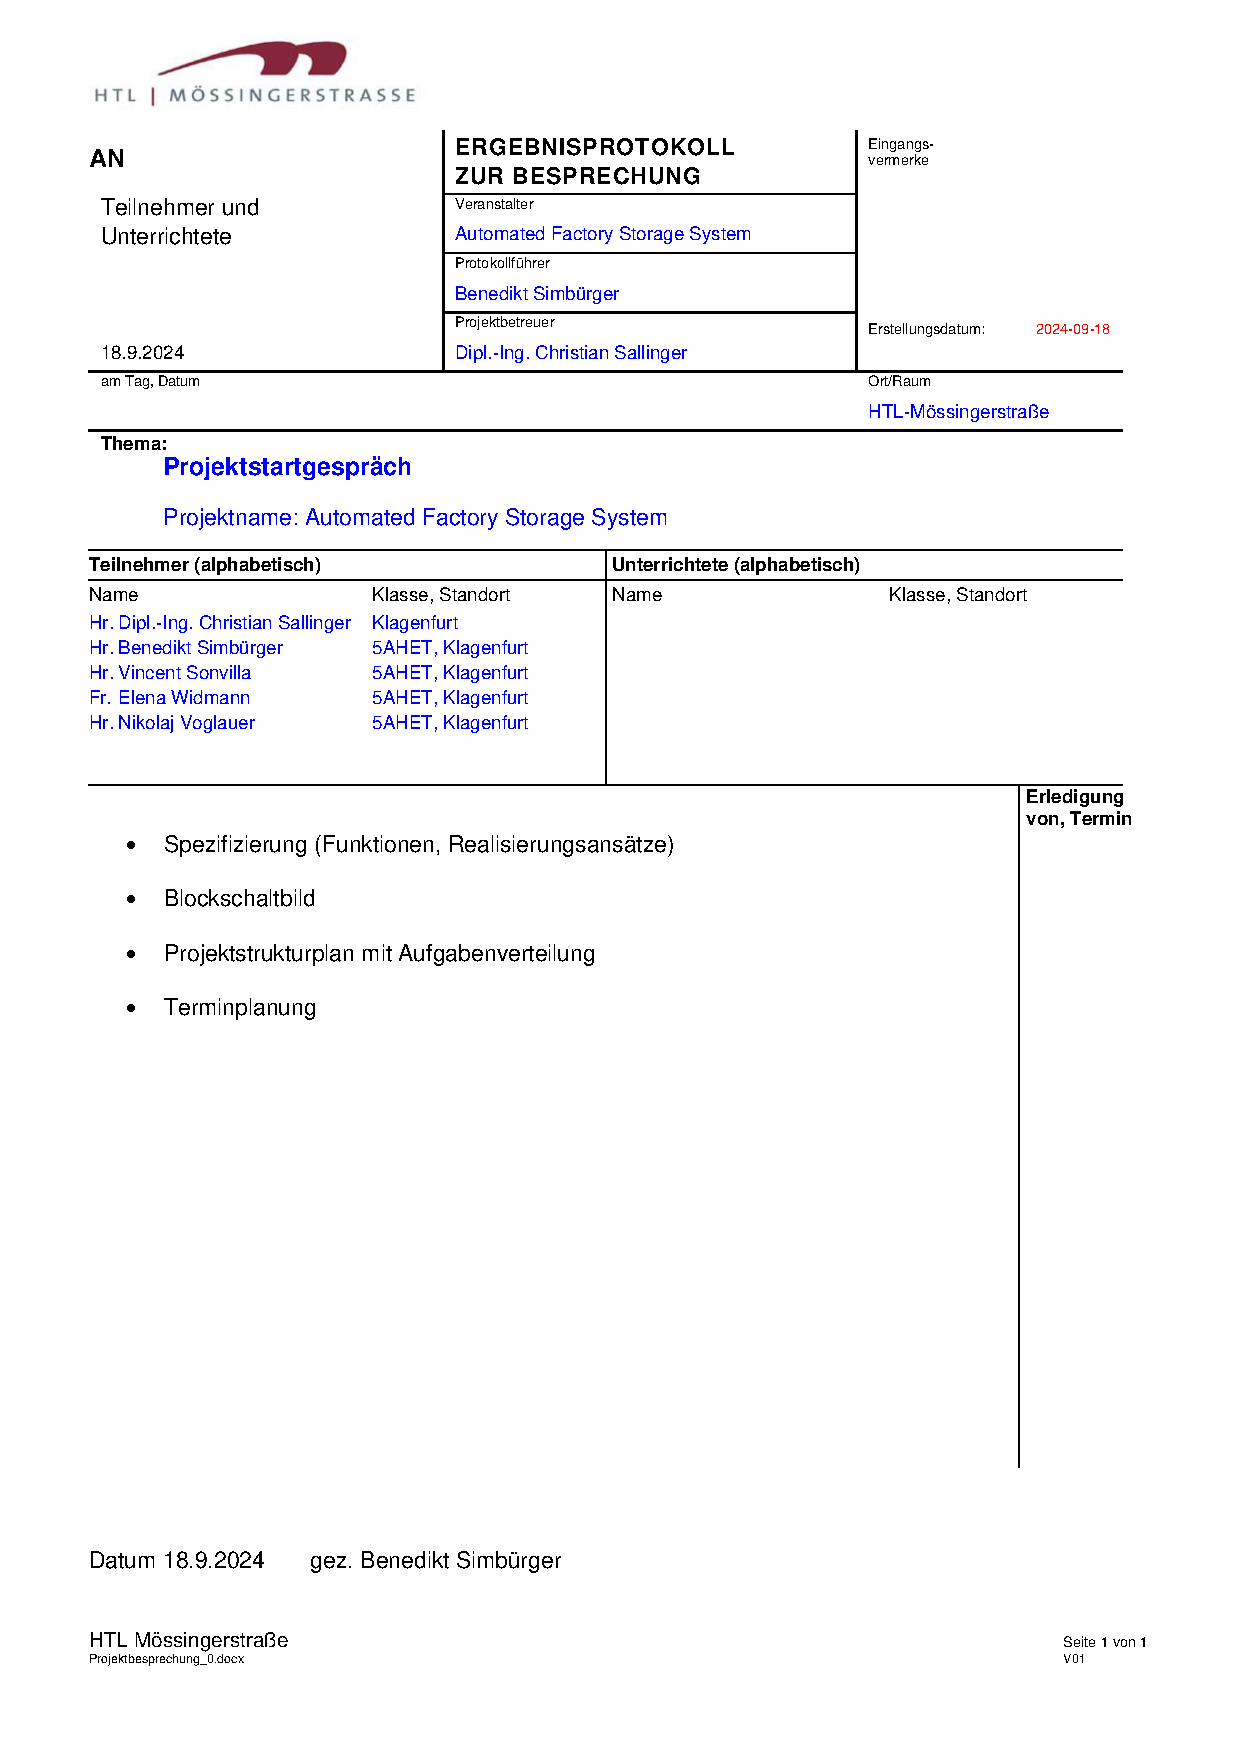
\includegraphics[width=0.9\textwidth]{../Protokolls/Projektbesprechung_0.pdf}
    \centering
    \caption{Besprechungsprotokoll 10.12.2024}
\end{figure}

\begin{figure}[H]
    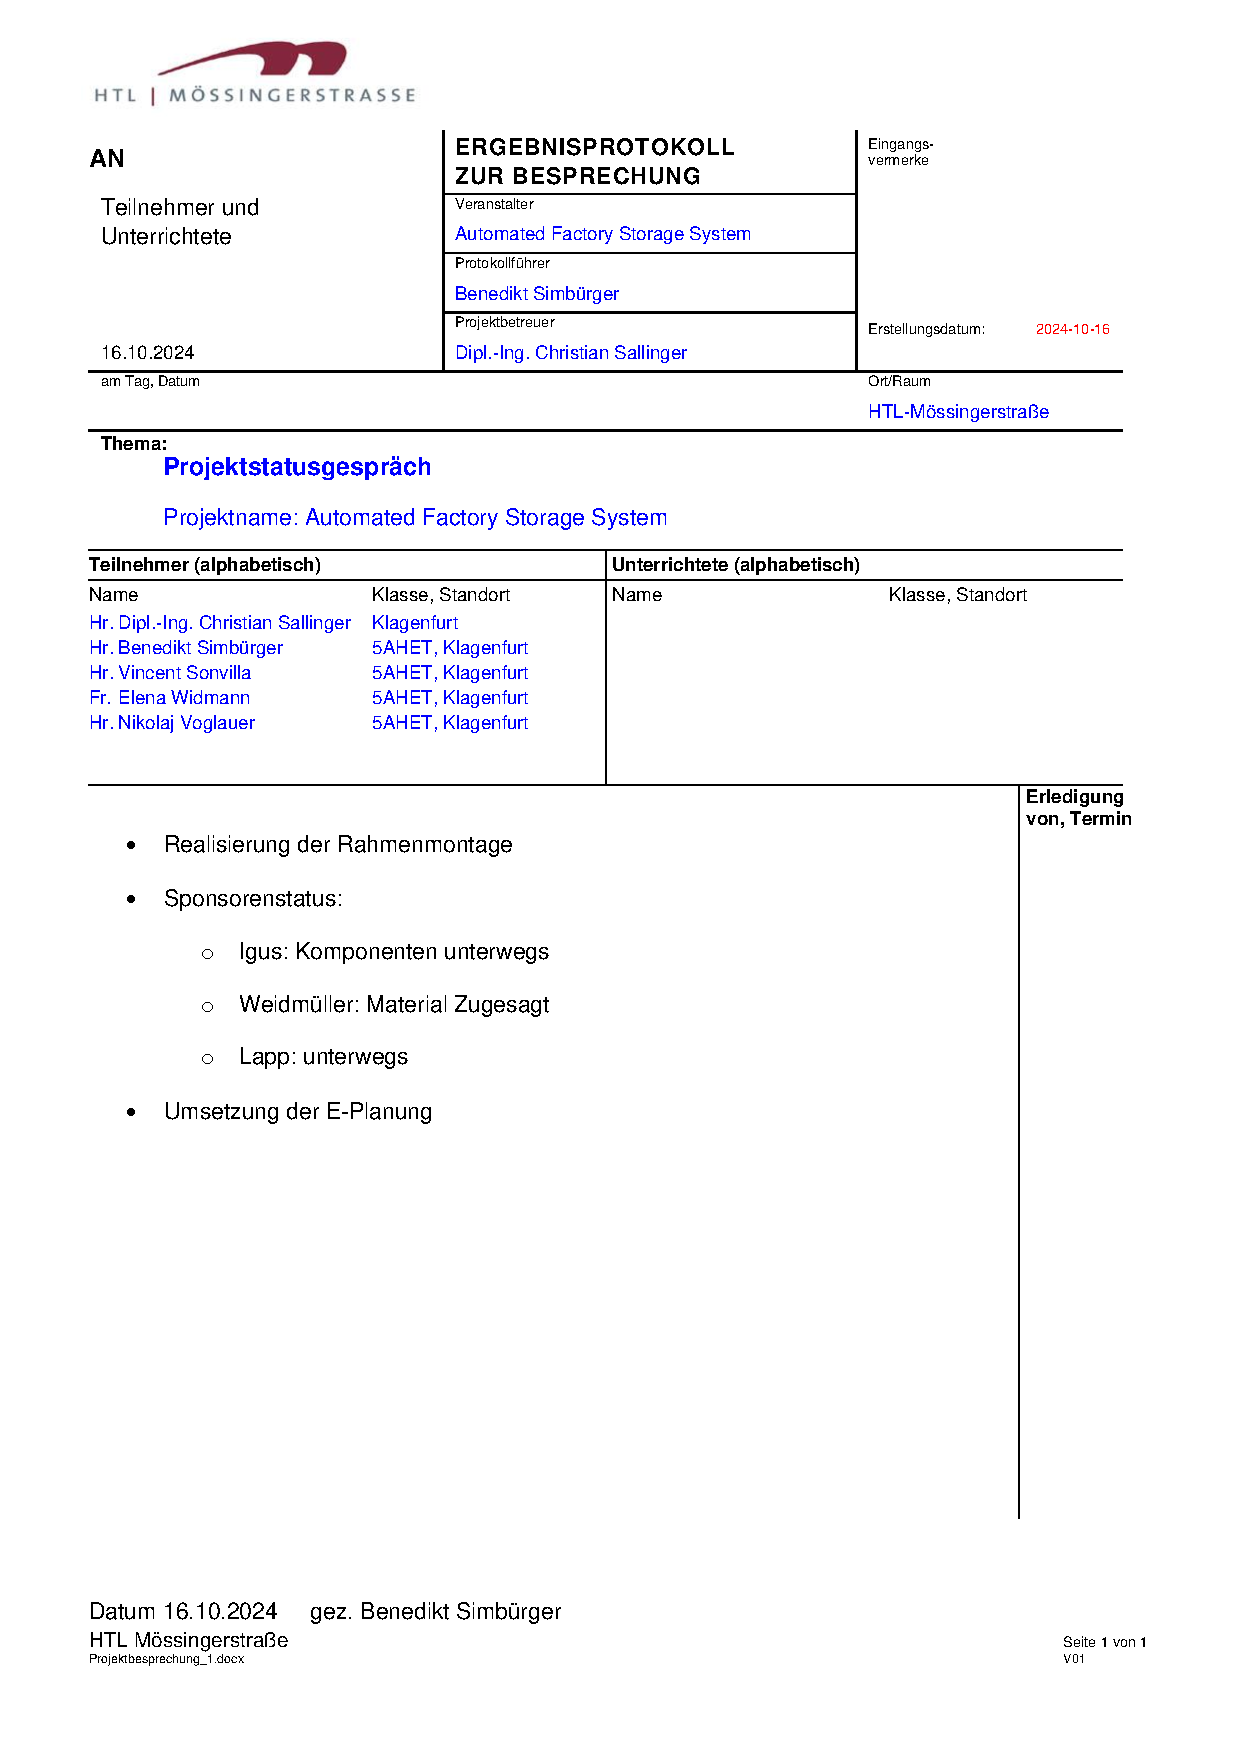
\includegraphics[width=0.9\textwidth]{../Protokolls/Projektbesprechung_1.pdf}
    \centering
    \caption{Besprechungsprotokoll 16.10.2024}
\end{figure}

\begin{figure}[H]
    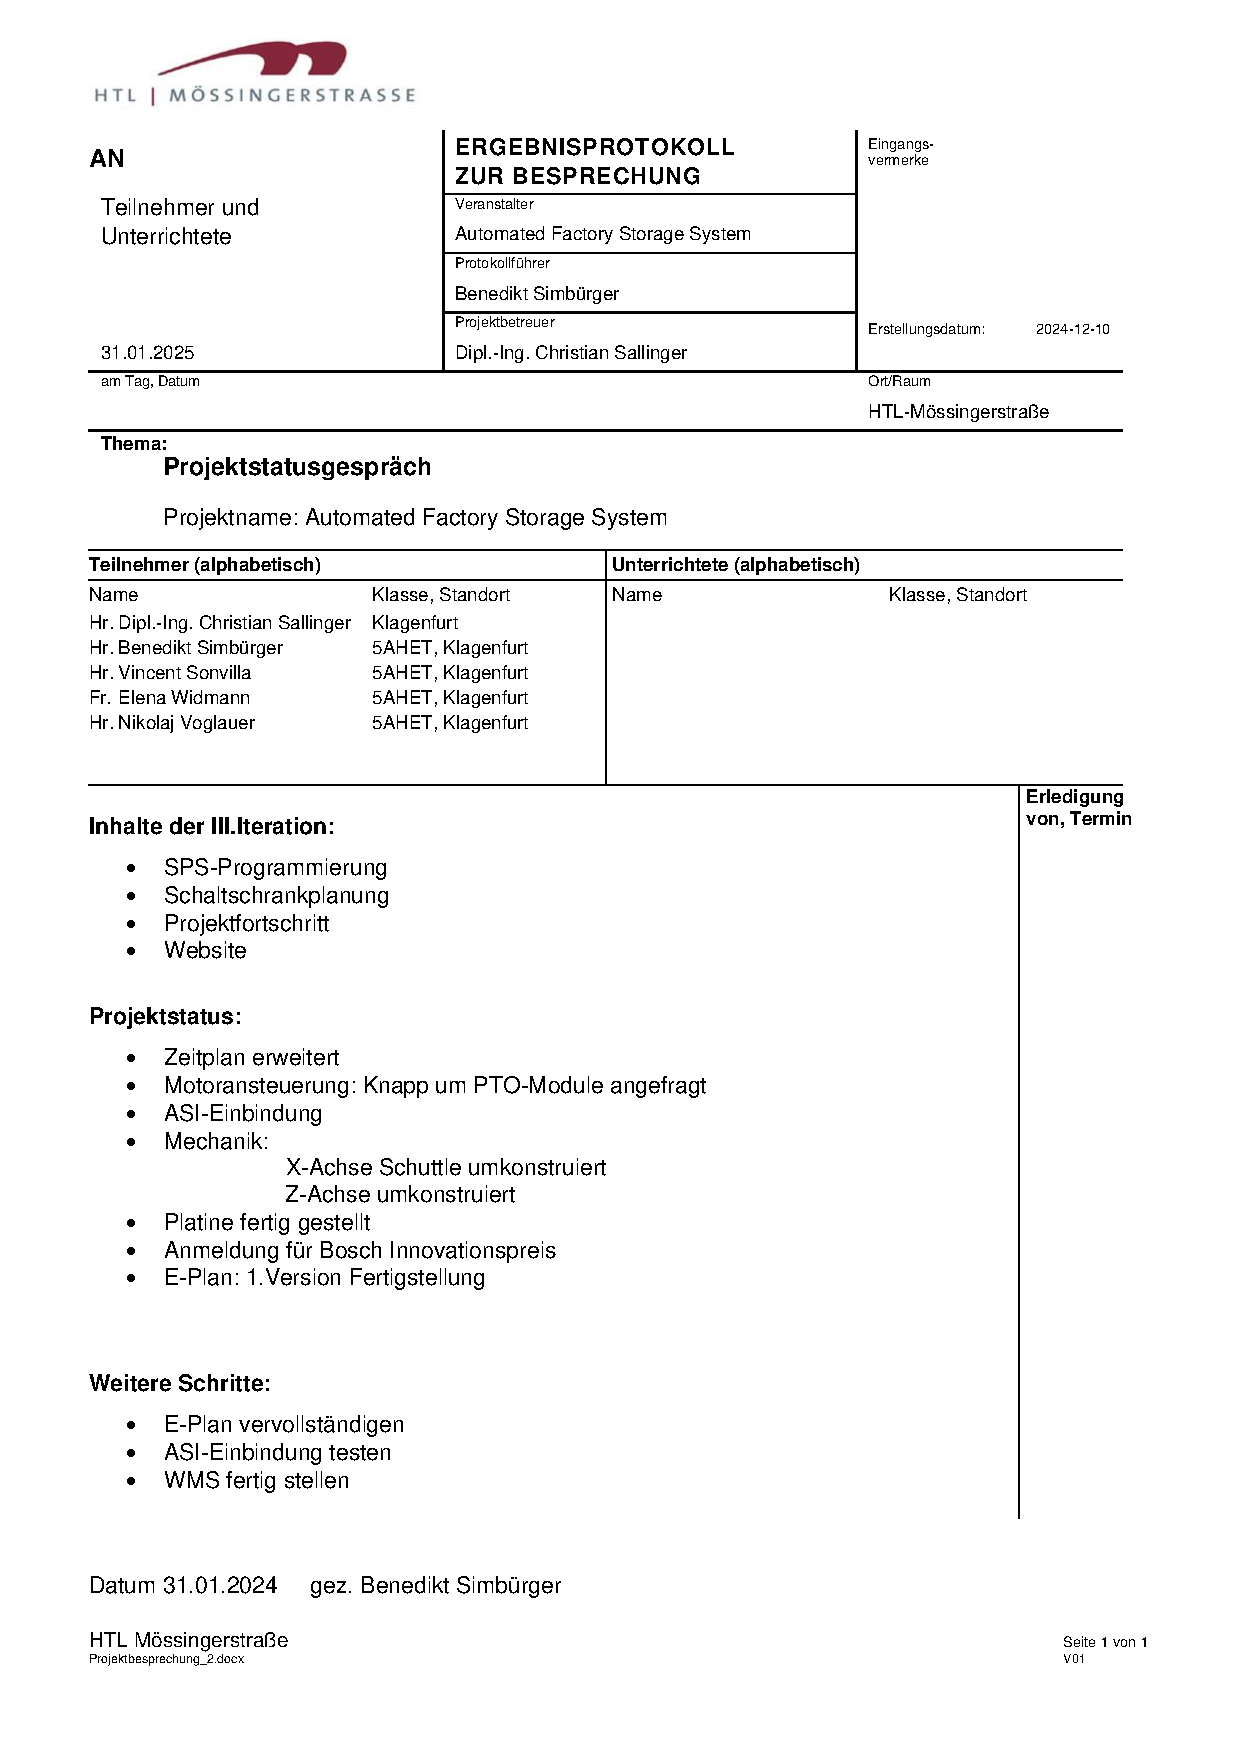
\includegraphics[width=0.9\textwidth]{../Protokolls/Projektbesprechung_2.pdf}
    \centering
    \caption{Besprechungsprotokoll 10.12.2024}
\end{figure}

\begin{figure}[H]
    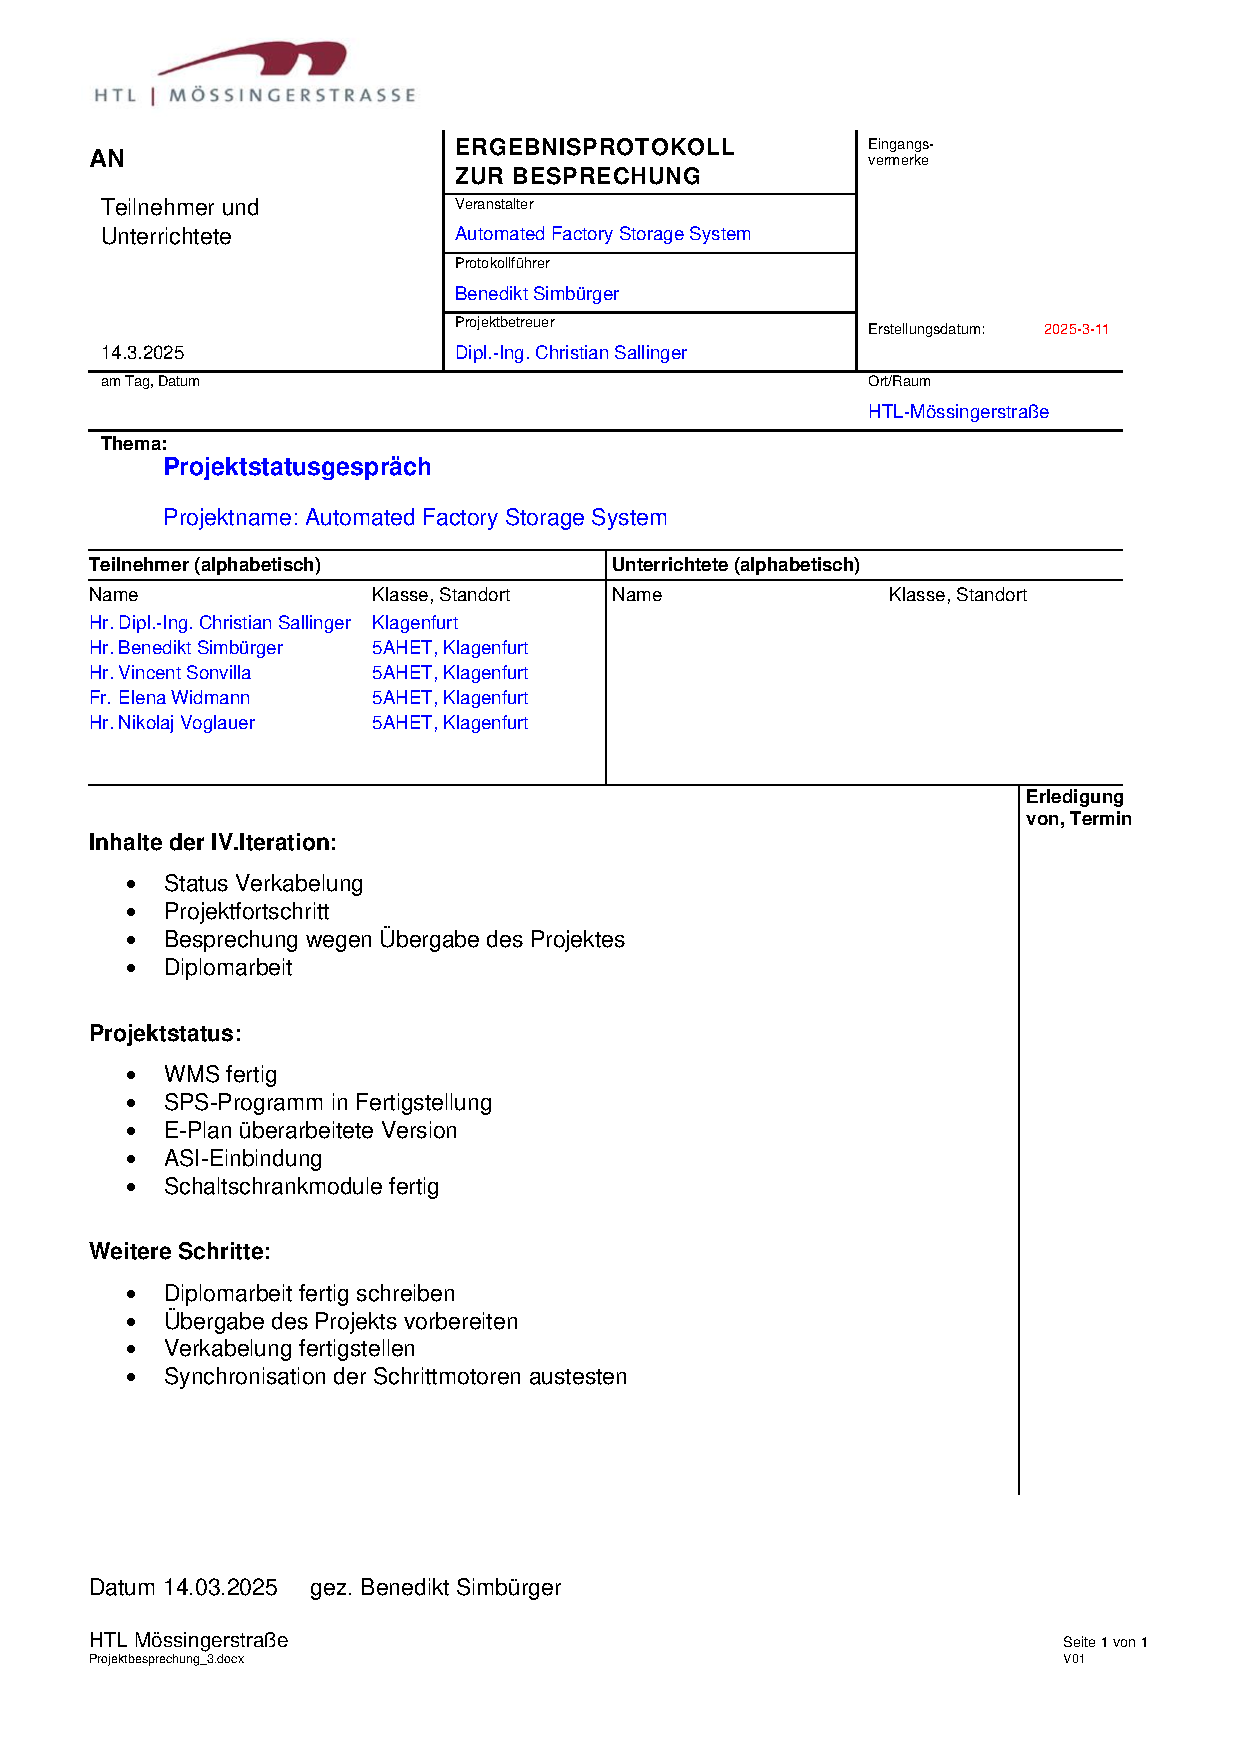
\includegraphics[width=0.9\textwidth]{../Protokolls/Projektbesprechung_3.pdf}
    \centering
    \caption{Besprechungsprotokoll x.x.xxxx}
\end{figure}




\newpage
\subsection{Arbeitsnachweis}
\textcolor{blue}{Jedes Teammitglied (Schüler/in) hat einen vollständigen Arbeitszeitnachweis, der außer-halb des Unterrichts verrichteten Tätigkeiten, in tabellarischer Form zu erbringen. \\Eine entsprechende Vorlage wird auf den Schulrechner in Form einer Excel-Vorlage bereitgestellt.}

\begin{longtable}{|l|p{10cm}|r|}
    \hline
    \textbf{Datum} & \textbf{Tätigkeit} & \textbf{Stunden} \\
    \hline
    \endfirsthead

    \hline
    \textbf{Datum} & \textbf{Tätigkeit} & \textbf{Stunden} \\
    \hline
    \endhead

    \hline
    \endfoot

    \hline
    \endlastfoot

4.10.2023	&Besprechung des weiteren vorgehens mit WB	&0.5\\
9.10.2023&	Gruppenbesprechung für das weitere Vorgehen	&1.0\\
9.11.2023&	Reconstruction Siemens Twin Towers	&3.5\\
14.11.2023&	Reconstruction Siemens Twin Towers	&2.0\\
23.11.2023&	Reconstruction Siemens Twin Towers Lasern	&2.0\\
29.11.2023&	RSTT Ausfahrer + Schlitten Fertig&	4.0\\
19.12.2023	&CAD Auf/Ab-fahrer	&3.0\\
20.12.2023	&CAD RSTT, AutCad vorbereitung	&2.0\\

10.1.2024	&Testversuch ET200 SPS Stepdrive inkl. Meeting Knapp&	4.0\\
11.1.2024	&Achse mech. fertig, Schlitten Vertikal&	4.0\\
12.1.2024	&CAD Schuttel, Tag der offenen Tür	&2.0\\

16.1.2024	&Motor ansteuern&	1.0	\\
20.1.2024	&Umlenkungen und Aufhängungskonstruktion&	4.0\\
29.1.2024	&Diagramm Datenaustausch	&2.0\\

1.2.2024	&Besprechung WB&	4.0\\
3.2.2024	&WS Backend/Frontend Prototyp&	9.0\\
4.2.2024	&WS Frontend&	3.0\\

5.2.2024	&KWF Antrag schreiben und WS Datenbankmanagement&	3.0\\
7.2.2024	&OPC UA Client&	4.5\\
15.2.2024	&WS Suche usw, Orga, Maschinenbaubesprechung	&5.5\\

20.2.2024	&Python / OPC UA Client 	&1\\
23.2.2024	&WS Warenkorb, restructuring	&9.0\\
24.2.2024	&WS Warenkorb fertig OPC anfang und Pflichtenheft Erstversion&	6.0\\
27.2.2024	&Barcode-Scanner/http-Kommunikation	&4.0\\
28.2.2024	&Lasten/Pflichtenheft erstellen	&3.0\\


4.3.2024	&Barcode-Scanner/http-Kommunikation&	3.5\\
10.3.2024	&CAD X-Achse	&7.0\\

13.3.2024	&Absprache mit Wurnitsch bez. Pflichtenheft	&1.0\\
14.3.2024	&Barcode-Scanner/http-Kommunikation/Fusion oder so&	3.0\\
1.4.2024	&Datenbanken und Visu	&5.0\\

2.4.2024	&Lagerregal&	2.0\\
17.4.2024	&Gabel und Software&	2.0\\
23.4.2024	&STT-Fortsetzung / Software einführung&	2.5\\
12.4.2024	&Datenbanken und Visu	&5.0\\
21.4.2024	&Datenbanken und Visu	&5.0\\
22.4.2024	&cooler search stuff	&3.0\\
23.4.2024	&cooler search stuff Implementierung	&2.0\\
28.4.2024	&Areas und Locations implementierung	&6.0\\
19.4.2024	&Order stuff	&3.0\\
22.5.2024	&Order algorithmus	&3.0\\
2.6.2024	&Order api	&5.0\\
3.6.2024	&Api implement und visu	&3.0\\

4.6.2024	&STT-Fortsetzung / CAD&	2.0\\
6.6.2024	&SPS/Server Communictaion und Z-Prototyp CAD	&5.0\\
8.6.2024	&SPS Comm und Simu implement	&4.0\\
9.6.2024	&System Controler	&4.0\\

14.6.2024	&Z-Prototyp Bauteile Vorbereitung&	1.0\\
18.6.2024	&Return, Cart	&4.0\\
19.6.2024	&Docker (f me)	&3.0\\

21.6.2024	&Z-PT, Schaltschrank, SPS-Com&	4.5\\
16.7.2024	&Recherche, Ref-Elektronik&	1.0\\
17.7.2024	&Ref-Elektronik	&2.0\\
19.7.2024	&Designe/CAD rollen u. spannen y, ...	&6.0\\
22.7.2024	&Designe X-Spann	&2.0\\
25.7.2024	&Design X-Spann, Rollen	&1.5\\
31.7.2024	&Z-Achsen zauberei (sike)(doch ned)&	1.0\\
1.8.2024	&Z-Achse Redesign (sigh)	&5.0\\
9.8.2024	&YZ-Achse grobe fertigstellung&	5.0\\
10.8.2024	&YZ-Achse feinerschliff	&4.0\\
11.8.2024	&YZ-Achse + X-Achse beginn&	2.0\\
12.8.2024	&X-Achse	&1.0\\
13.8.2024	&X-Achse side roller	&4.0\\
14.8.2024	&X-Achse side roller 2. side	&2.0\\
15.8.2024	&X-Achse Mid rollers, side wheeles 90, yz-achse spiegelung	&6.0\\
16.8.2024	&YZ-Achse lichttaster, X-Achse	&1.0\\
17.8.2024	&X-Achse Schleppkettengedanken 	&6.0\\
19.8.2024	&Schleppenderketten	&2.0\\
20.8.2024	&Vertikeale Schleppkette	&3.0\\
20.8.2024	&Sponsorenemail beginn	&1.3\\
21.8.2024	&Kontaktdaten, Projektzusammenfassung	&1.5\\
22.8.2024	&Schlitten Top	&1.0\\
24.8.2024	&Stückliste, Schlitten Top	&2.0\\
25.8.2024	&X-Top Verbindung, Umlenkung	&5.0\\
27.8.2024	&Rahmen aufhängungen	&2.0\\
29.8.2024	&Umlenkungen, Motoraufhängungen	&5.0\\
30.8.2024	&Endschalter, Rahmen beginn	&3.0\\
31.8.2024	&Rahmen, Lagerschrank beginn	&6.0\\
1.9.2024	&Lagerschrank, Querfördererauschschnitt	&2.0\\
2.9.2024	&Bissi Software angeschaut wieder, cooler slider	&1.0\\
3.9.2024	&Software Richten, Weidmüller Sortiment Bauteile auswählen	&4.0\\
4.9.2024	&Stack Bug behoben, Querförderer	&7.0\\
5.9.2024	&Mech weitestgehende Fertigstellung	&4.0\\
9.9.2024	&Marketing, Fortschritts-Leafletter (+ Latex aufsetzen)	&2.5\\

10.9.2024	&Meeting Weidmüller&	2.0	\\
11.9.2024	&Schaltschrank konzeptionierung (Materialliste fast vollständig)	&2.25\\


15.9.2024	&Lapp Liste, Knapp Update, Fusion Stücklistenanfänge	&2.0\\

17.9.2024	&Autolager Demontieren für Bauteilbeschaffung&	2.5\\
18.9.2024	&Förderband Abmessen, Verbindungstest, Sensorensicherun, Suchalgorythmus Rustimplementation &6.0\\
19.9.2024	&Suchag. Fertig implementiert. Rollen gezeichnet	&3.0\\

24.9.2024	&Projektmanagement&	3.0\\
25.9.2024	&Änderungen V-Slot-Aufhängung, Project-Libre	&1.0\\

26.9.2024	&Igus, Weidmüller, Motoren ansteuern die 1.&	4.0\\
28.9.2024	&Bux im Lageralgo beheben	&1.5\\

1.10.2024	&Zeitplan, Sensoren recherchieren, SchSch-Konzept. CAD	&1.0\\
3.10.2024	&Profile bearbeiten	&1.5\\
8.10.2024	&Latex Vorlage	&1.0\\
9.10.2024	&Raumeinrichtung, SchSch Komzept&	3.0\\
21.10.2024	&Rahmenbau beginn&	2.0\\
22.10.2024	&Rahmenbauu + Drehstrom, 2.Präsentation, Auftragsvorbereitung X-Aufhängung, Referenzschaltung &5.5\\
23.10.2024	&Rahmenbau	&3.0\\
24.10.2024	&Rahmenbau, Poster/2.Präsentation	&3.0\\
25.10.2024	&XZ-Redesign	&3.0	\\
26.10.2024	&XZ-Redesign	&7.0	\\
27.10.2024	&Auftragsvorbereitung X-Achse	&3.0\\
28.10.2024	&Auftragsvorbereitung X-Achse	&2.0	\\

5.11.2024	&Beginn Umlenkrollen Drehen	&0.8\\
6.11.2024	&Weidmüller DP Inbetrtiebnahme&	1.0\\
7.11.2024	&E-Plan/Autocad, Weidmülller ansteuern&	3.5\\
8.11.2024	&E-Plan/Autocad, Weidmülller ansteuern&	3.5\\
12.11.2024	&Drehen, E-Plan, &	3.5\\
19.11.2024	&Drehen, Fräsen	&2.5\\
20.11.2024	&DAS Beg drehen	&1.0\\
21.11.2024	&DAS TFIDF	&2.0\\
22.11.2024	&Eplan, Website, SPS, Dipl Arbeit	&4.5\\
23.11.2024	&API stack umscheissen, DPWS	&3.0\\
24.11.2024	&DPWS	&2.0\\
25.11.2024	&DPWS	&1.5\\

26.11.2024	&Eplan, Website, SPS, Drehen& 3.5\\
29.11.2024	&Eplan, Website/Referenzplatine, Blockschaltbild, Dipl Arbeit& 4.0\\
3.12.2024	&Drehen,ASI-Sensoren-Platine, Diplomarbeit, DA Maschinenbau& 5.0\\
6.12.2024	&Website, DA &3.5\\
10.12.2024	&DA, Fusion, ASi in E-Plan, DA software	&5.0\\
13.12.2024	&E-Plan &3.5\\
7.1.2025	&Website, SchSch, SPS, CNC-Fräsen, Hülsen Drehen&	3.5\\
8.1.2025	&X-Achse Zusammenbauen anfangen	&2.0\\
10.1.2025	&CAD für Schaltschrankmodule, ZB	&4.0\\
14.1.2025	&Zusammenbauen, SPS, …&	4.0\\
15.1.2025	&ZB, Kabel verlegen, Platinen löten&	4.5\\
17.1.2025	&Tag der offenen Türe	&5.0\\
21.1.2025	&Schaltschrank, TIA Portal, ?&	3.5\\
24.1.2025	&Lasern, Förderband, Mechanik	&3.5\\
4.2.2025	&Sicherheitstechnik-Besprechung, SPS <--> Server	&3.5\\
14.2.2025	&WMS Location Updateing	&1.0\\
17.2.2025	&DA allgem	&1.0\\

21.2.2025	&Ref, Fräsen, Da-Schreiben	&5.0\\
25.2.2025	&Zusammenbauen&	4.0\\
28.2.2025	&Fräsen, E-Plan,&	3.5\\
2.3.2025	&DA aufbau	&1.5\\
3.3.2025	&DA - Besprechungsprotokolle&	1.0\\

5.3.2025	&Umlenkung + Motoren&	4.5\\
6.5.2025	&DA-Schreiben  &	2.5\\
9.3.2025	&DA - yz	&1.0\\

10.3.2025	&DA-schrieben	&3.0\\
11.3.2025	&DA-schreiben	&3.0\\
14.3.2025	&Verkabelung Schaltschrank	&4.0\\


    
\end{longtable}


\newpage
